% Copyright 2023  Ed Bueler

\documentclass[10pt,
               svgnames,
               hyperref={colorlinks,citecolor=DeepPink4,linkcolor=FireBrick,urlcolor=Maroon},
               usepdftitle=false]{beamer}

\mode<presentation>
{
  \usetheme{Madrid}

  \usecolortheme{beaver}

  \setbeamercovered{transparent}
  
  \setbeamerfont{frametitle}{size=\large}
}

\setbeamercolor*{block title}{bg=red!10}
\setbeamercolor*{block body}{bg=red!5}

\usepackage[english]{babel}
\usepackage[latin1]{inputenc}
\usepackage{times}
\usepackage[T1]{fontenc}
% Or whatever. Note that the encoding and the font should match. If T1
% does not look nice, try deleting the line with the fontenc.

\usepackage{empheq,bm,xspace,minted}
\usepackage{hyperref}
\usepackage{tikz}

% If you wish to uncover everything in a step-wise fashion, uncomment
% the following command: 
%\beamerdefaultoverlayspecification{<+->}

\newcommand{\bb}{\mathbf{b}}
\newcommand{\bc}{\mathbf{c}}
\newcommand{\bbf}{\mathbf{f}}
\newcommand{\bl}{\bm{\ell}}
\newcommand{\br}{\mathbf{r}}
\newcommand{\bs}{\mathbf{s}}
\newcommand{\bx}{\mathbf{x}}
\newcommand{\by}{\mathbf{y}}
\newcommand{\bv}{\mathbf{v}}
\newcommand{\bu}{\mathbf{u}}
\newcommand{\bw}{\mathbf{w}}

\newcommand{\bzero}{\bm{0}}

\newcommand{\CC}{\mathbb{C}}
\newcommand{\RR}{\mathbb{R}}

\newcommand{\ddt}[1]{\ensuremath{\frac{\partial #1}{\partial t}}}
\newcommand{\ddx}[1]{\ensuremath{\frac{\partial #1}{\partial x}}}
\renewcommand{\t}[1]{\texttt{#1}}
\newcommand{\Matlab}{\textsc{Matlab}\xspace}
\newcommand{\Octave}{\textsc{Octave}\xspace}
\newcommand{\eps}{\epsilon}

\newcommand{\twovect}[4]{\ensuremath{{#1}_{#2} =
                            \begin{bmatrix} #3 \\ #4 \end{bmatrix}}}

\newcommand{\ftt}[1]{{\color{blue} \texttt{#1}}}

\newcommand{\optimaldef}{
\begin{definition}
an algorithm for computing a function on a class of problems, which acts on floating-point data of size $N$, is \emph{optimal} if it requires
   $$O(N) \qquad \text{ or } \qquad O(N\log N) \qquad \text{ flops}$$
as $N\to\infty$
\end{definition}
}



\title{Optimal solvers for partial differential equations}

\subtitle{With parallel scaling too!}

\author{Ed Bueler}

\institute[]{UAF Math 692 Scalable Seminar}

\date{Spring 2023}


\begin{document}
\beamertemplatenavigationsymbolsempty

\begin{frame}
  \maketitle
\end{frame}

\begin{frame}{Outline}
  \tableofcontents[hideallsubsections]
\end{frame}

\section{x}


\begin{frame}{x}
\begin{itemize}
\item x
\end{itemize}
\end{frame}


\begin{frame}[fragile]
\frametitle{\texttt{matvec}}
\begin{itemize}
\item y
\end{itemize}
\begin{center}
\begin{minipage}{0.7\textwidth}
\begin{minted}[fontsize=\small]{python}
def matvec(A,x):
    from numpy import zeros, shape
    [m,n] = shape(A)
    z = zeros((m,1))
    for i in range(m):
        s = 0.0
        for j in range(n):
            s += A[i][j] * x[j]
        z[i] = s
    return z
\end{minted}
\end{minipage}
\end{center}
\end{frame}


\begin{frame}{references}

\begin{columns}
\begin{column}{0.8\textwidth}
\begin{itemize}
{\small
\item[] \textbf{A.~Brandt (1977)}. \emph{Multi-level adaptive solutions to boundary-value problems}, Mathematics of Computation 31 (138), 333--390
    \begin{itemize}
    \item[$\circ$] the guru of multigrid should be better known
    \end{itemize}
\item[] \textbf{W.~Briggs, V.~E.~Henson, \& S.~McCormick (2000)}.  \emph{A Multigrid Tutorial}, 2nd ed., SIAM Press, Philadelphia
\item[] \textbf{E.~Bueler (2021)}. \emph{PETSc for Partial Differential Equations}, SIAM Press, Philadelphia
    \begin{itemize}
    \item[$\circ$] Krylov methods, multigrid, optimal PDE solvers
    \end{itemize}
\item[] \textbf{U.~Trottenberg, C.~Oosterlee, \& A. Schuller (2001)}.  \emph{Multigrid}, Elsevier, Oxford
}
\end{itemize}
\end{column}
\begin{column}{0.17\textwidth}
\hfill 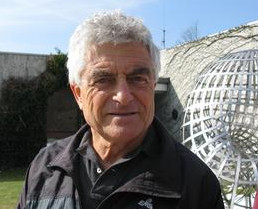
\includegraphics[width=\textwidth]{images/abrandt.jpg}

\vspace{7mm}
\hfill 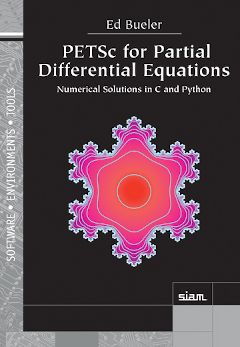
\includegraphics[width=0.8\textwidth]{images/bueler.jpg}
\end{column}
\end{columns}
\end{frame}

\end{document}
